\documentclass[a4paper,11pt]{article}

%----------------------------------------------
%	PACKAGE SPECS
%----------------------------------------------
\usepackage[czech]{babel}
\usepackage[utf8]{inputenc} % for correct characters
\usepackage[T1]{fontenc}
\usepackage{graphicx} % using pictures
\usepackage[dvipsnames]{xcolor} % colored text
\usepackage{indentfirst}
\usepackage{caption}
\usepackage[cache=false]{minted}

%----------------------------------------------
%	ENVIRONMENT SPECS
%----------------------------------------------
\newenvironment{bottompar}{\par\vspace*{\fill}}{\clearpage}

\setlength{\parindent}{2em}
\graphicspath{ {images/} }

\renewcommand\listingscaption{Příklad}

%----------------------------------------------
%	AUTHOR AND FILE INFO
%----------------------------------------------
\title{IPK Projekt 2, DHCP Starvation útok}
\author{Daniel Dolejška}
\date{Duben 2018}

%----------------------------------------------
%	CONTENTS
%----------------------------------------------
\begin{document}

%------------------
%	Title page
%------------------
\begin{titlepage}
\centering

\huge\textbf{IPK Projekt 2}

\vspace{5mm}

\large Varianta 2: DHCP Starvation útok

\vfill

\large Daniel Dolejška \textsf{(xdolej08)}

\vspace{2mm}

\small Duben 2018

\vspace{1cm}


\includegraphics[width=6cm]{vutbr-fit.png}

\end{titlepage}

%------------------
%	ToC
%------------------
\newpage
\tableofcontents
\listoffigures


%------------------
%	Page: Teorie útoku
%------------------
\newpage
\section{Teorie útoku} \label{teorie}

V této sekci je popsána teorie a princip DHCP starvation útoku a k čemu jej lze využít.

\subsection{Princip útoku}

Cílem útoku je simulovat v síti zařízení žádající o přiřazení IP adresy (popř. dalšího síťového nastavení) a vyčerpat tak množinu adres, kterou má místní DHCP server/servery k dispozici.

\vspace{2mm}
Útočník poté může spustit svůj vlastní DHCP server a uživatelům přidělovat legitimní síťové adresy, které získal. Následně může, díky plné kontrole nad přiděleným nastavením, směrovat síťový provoz dle libosti a dospět tak k dalšímu typu útoku - \textbf{MITM, man-in-the-middle attack}.

\subsection{Zprostředkování útoku}

Útočící aplikace provede za pomoci \textbf{MAC spoofing} odeslání \mbox{\textsf{DHCPDISCOVER}} packetu s podvrženou MAC adresou. Vyčká na odpověď DHCP serveru ve formě \mbox{\textsf{DHCPOFFER}} packetu, který následně potvrdí pomocí \mbox{\textsf{DHCPREQUEST}} packetu. Celý proces je dokončen ve chvíli, kdy útočící aplikace obdrží \mbox{\textsf{DHCPACK}}.

\vspace{2mm}
Celý tento proces může aplikace opakovat, dokud množinu přiřaditelných adres legitimního DHCP serveru nevprázdní.

\vspace{2mm}
Útočící aplikace následně může začít odpovídat na DHCP broadcasty zařízení namísto legitimního DHCP serveru a nabízet získané IP adresy s podvrženým síťovým nastavením.

%\vfill
%\hrule
%\vspace{1mm}\noindent


%------------------
%	Page: Implementace
%------------------
\newpage
\section{Implementace} \label{implementace}

Tato sekce obsahuje informace o mé implementaci útočící aplikace.

\subsection{Soubory aplikace}

Aplikace je rozdělena do několika souborů v několika kategoriích, kde se každá kategorie stará pouze o svou oblast:

\begin{description}
	\item [Hlavní program] Obsahuje hlavní řídící program, využívající funkce z ostatních souborů projektu, implementující funkcionalitu DHCP starvation útoku.
	\begin{itemize}
		\item \textsf{main.c}
	\end{itemize}

	\item [DHCP] Obsahuje funkce zajišťující práci s daty protokolu DHCP v přijatém packetu, dále zajišťují možnost vytváření těchto packetů, validaci dat a jejich jednoduchou modifikaci.
	
	Část obsahu tohoto souboru (definice datové struktury protokolu a definice konstantních hodnot) byla převzata od Internet Systems Consortium, Inc.
	\begin{itemize}
		\item \textsf{dhcp.h}
		\item \textsf{dhcp.c}
	\end{itemize}

	\item [Síť] Obsahuje funkce zajišťující práci s daty ethernetové hlavičky, hlavičky protokolu IP a UDP, dále zajišťují možnost vytváření těchto dat v packetech, validaci dat a jejich jednoduchou modifikaci.
	\begin{itemize}
		\item \textsf{network.h}
		\item \textsf{network.c}
	\end{itemize}

	\item [Obecné funkce] Obsahuje několik jednoduchých funkcí pro náhodné generování čísel a MAC adres.
	\begin{itemize}
		\item \textsf{general.h}
		\item \textsf{general.c}
	\end{itemize}
\end{description}

\subsection{Posloupnost akcí}

\begin{enumerate}
	\item Příprava před prvotním odesíláním
	
	V této chvíli aplikace generuje náhodnou MAC adresu a vytváří hlavičky datagramu pro broadcast.
	
	
	\item Odesílání \textsf{DHCPDISCOVER}
	
	Aplikace přidá za vytvořené hlavičky do datagramu potřebná data DHCP protokolu a ten následně odešle.
	
	
	\item Příjem \textsf{DHCPOFFER}
	
	Při příjmu datagramů probíhá kontrola \textit{IP adresy zdroje}, \textit{atributu \textsf{chaddr}, \textsf{xid} a \textsf{op} DHCP protokolu} a v neposlední řadě \textit{option \textsf{0x35 (message type)} DHCP protokolu}.
	
	Na základě výsledků kontrol bud probíhá krok číslo 3 znovu (příjem dalšího datagramu), nebo se pokračuje ve zpracování dalším krokem.
	
	V případě nepřijetí žádného datagramu protokolu DHCP se aplikace po několika sekundách vrací na krok číslo 2 a opakuje odeslání \textsf{DHCPDISCOVER} datagramu. Při opakovaném neúspěchu stejného typu je aplikace ukončena.
	
	
	\item Odesílání \textsf{DHCPREQUEST}
	
	Probíhá vytvoření a odeslání odpovědi na přijatý \textsf{DHCPOFFER} datagram.
	
	
	\item Příjem \textsf{DHCPACK}
	
	Při příjmu datagramů probíhají stejné kontroly jako při kroku 3. Pokud se jedná o datagram požadovaného typu je IP adresa vypsána na \textsf{stdout} a označena za získanou.
	
	\textit{Aplikace dále pokračuje znovu bodem 1.}
\end{enumerate}


%------------------
%	Page: Demonstrace činnosti
%------------------
\newpage
\section{Demonstrace činnosti} \label{demonstrace}

\subsection{Spuštění aplikace}

Aplikace má povinný přepínač \textsf{-i} s názvem síťového rozhraní, ze kterého bude aplikace odesílat kompromitující data do sítě.

\mint{console}|isa2015@isa2015:/media/sf_ipk$ sudo ./ipk-dhcpstarve -i <interface>|

\small \textit{Podrobnější informace k spuštění aplikace či překladu zdrojových souborů jsou k dispozici v \textsf{README.md} souboru.} \normalsize

\subsection{Útok na malou domácí síť}

V této sekci jsou uvedeny příklady použití aplikace v domácím prostředí malé sítě (diagram sítě viz Obrázek \ref{fig:domaci-sit}). Součástí jsou i příklady časové náročnosti implementovaného řešení za různé velikosti množiny přiřaditelných adres DHCP serveru (\textsf{DHCP pool}).

\begin{figure}[H]
	\centering
	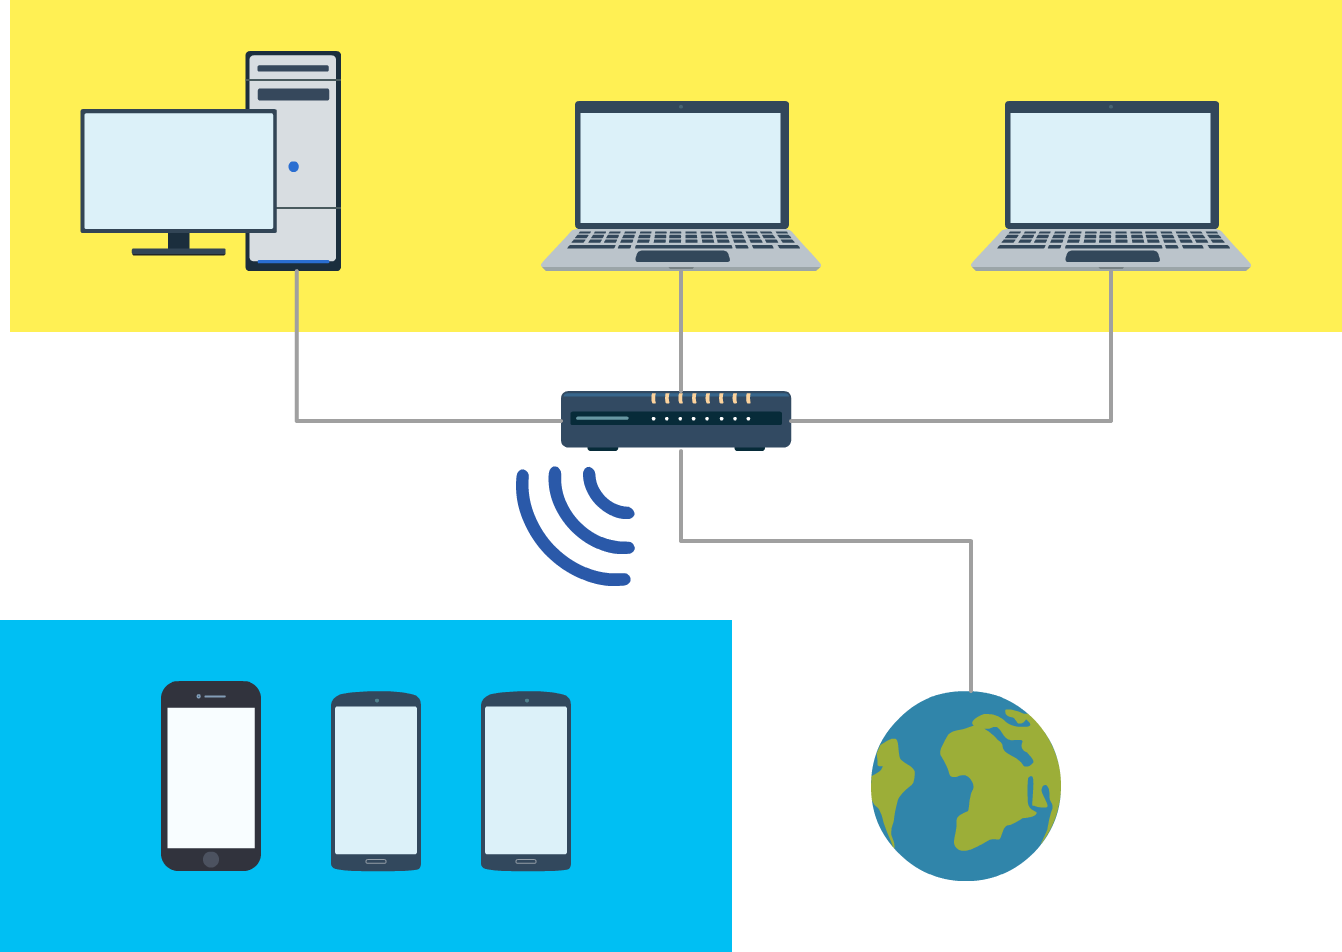
\includegraphics[width=7cm]{network-diagram.png}
	\caption[Diagram použité sítě]{Diagram použité sítě}
	\label{fig:domaci-sit}
\end{figure}

V příkladu číslo \ref{lst:demo-domaci} je ukázka jednoduchého použití aplikace. \small \textit{Podrobnější informace k spuštění aplikace či překladu zdrojových souborů jsou k dispozici v \textsf{README.md} souboru.} \normalsize

\begin{listing}[H]
	\begin{minted}{console}
isa2015@isa2015:/media/sf_ipk$ sudo ./ipk-dhcpstarve -i eth0
192.168.0.100
192.168.0.101
...
192.168.0.108
192.168.0.109
isa2015@isa2015:/media/sf_ipk$
	\end{minted}
	\centering
	\caption[Útok na domácí síť]{Výstup aplikace při použití v malé síti}
	\label{lst:demo-domaci}
\end{listing}

Zmocnění se desíti adres v malé domácí síti trvala zhruba 28 vteřin. Z toho ~16 vteřin je konečný timeout. Příklad použití a výstupů viz \listingscaption\space\ref{lst:demo-domaci10-cas}.

\begin{listing}[H]
	\begin{minted}{console}
isa2015@isa2015:/media/sf_ipk$ time sudo ./ipk-dhcpstarve -i eth0
192.168.0.100
...
192.168.0.109

real	0m27.878s
user	0m0.000s
sys	 0m0.008s
isa2015@isa2015:/media/sf_ipk$
	\end{minted}
	\centering
	\caption[Rychlost získání 10 adres]{Výstup aplikace při měření času a získávání 10 adres v malé síti}
	\label{lst:demo-domaci10-cas}
\end{listing}

Příklad časové náročnosti se zmocněním se 150 adres ve stejné síti viz \listingscaption\space\ref{lst:demo-domaci150-cas}.

\begin{listing}[H]
	\begin{minted}{console}
isa2015@isa2015:/media/sf_ipk$ time sudo ./ipk-dhcpstarve -i eth0
192.168.0.100
...
192.168.0.249

real	2m46.688s
user	0m0.000s
sys	 0m0.040s
isa2015@isa2015:/media/sf_ipk$ 
	\end{minted}
	\centering
	\caption[Rychlost získání 150 adres]{Výstup aplikace při měření času a získávání 150 adres v malé síti}
	\label{lst:demo-domaci150-cas}
\end{listing}

Všechny příklady uvedené v této sekci provedeny za použití výchozího nastavení (více o možnostech a výchozím nastavení viz soubor \textsf{README.md}).

\end{document}